\documentclass[tikz]{standalone}

\usepackage{circuitikz}

\begin{document}
	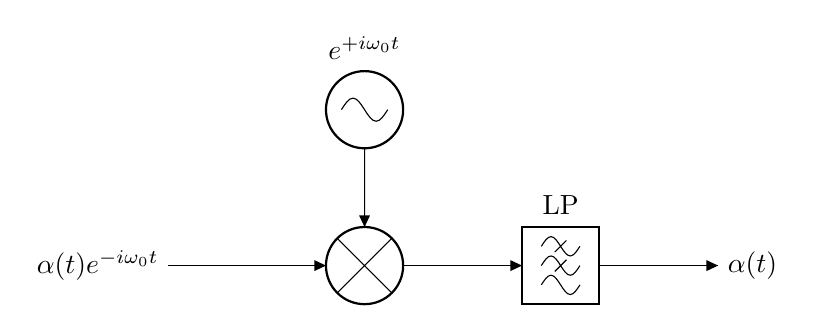
\begin{tikzpicture}
		\draw (0,0) node[left]{$\alpha(t)e^{-i\omega_0t}$} (2,0)
            node[mixer, anchor=west](mixer){};
		\draw (0,0) to[short] (mixer.west);
        \node [inputarrow, anchor=tip] at (mixer.west) {};
        \draw (mixer.east) to[lowpass, >, l=LP] ++(4,0) to[short] ++(0,0) node[inputarrow]{} node[right]{$\alpha(t)$};
        \draw (mixer.north) node[inputarrow, rotate=-90]{} to[short] ++(0,1) node[oscillator, anchor=south](osc){} ++(0,1) node[above]{$e^{+i\omega_0t}$};
	\end{tikzpicture}
\end{document}